\documentclass{article}

% Any packages or configurations specific to this section
\usepackage{lipsum}
\usepackage{graphicx}

\begin{document}

\section{Results}

Using ENApp, the 
\subsection*{Various Analyses on IEEE 123 Node System in a 5 Hour Horizon}

\begin{figure*}[h!]
    \centering
    % Row 1
    \begin{subfigure}[b]{0.3\textwidth}
        \centering
        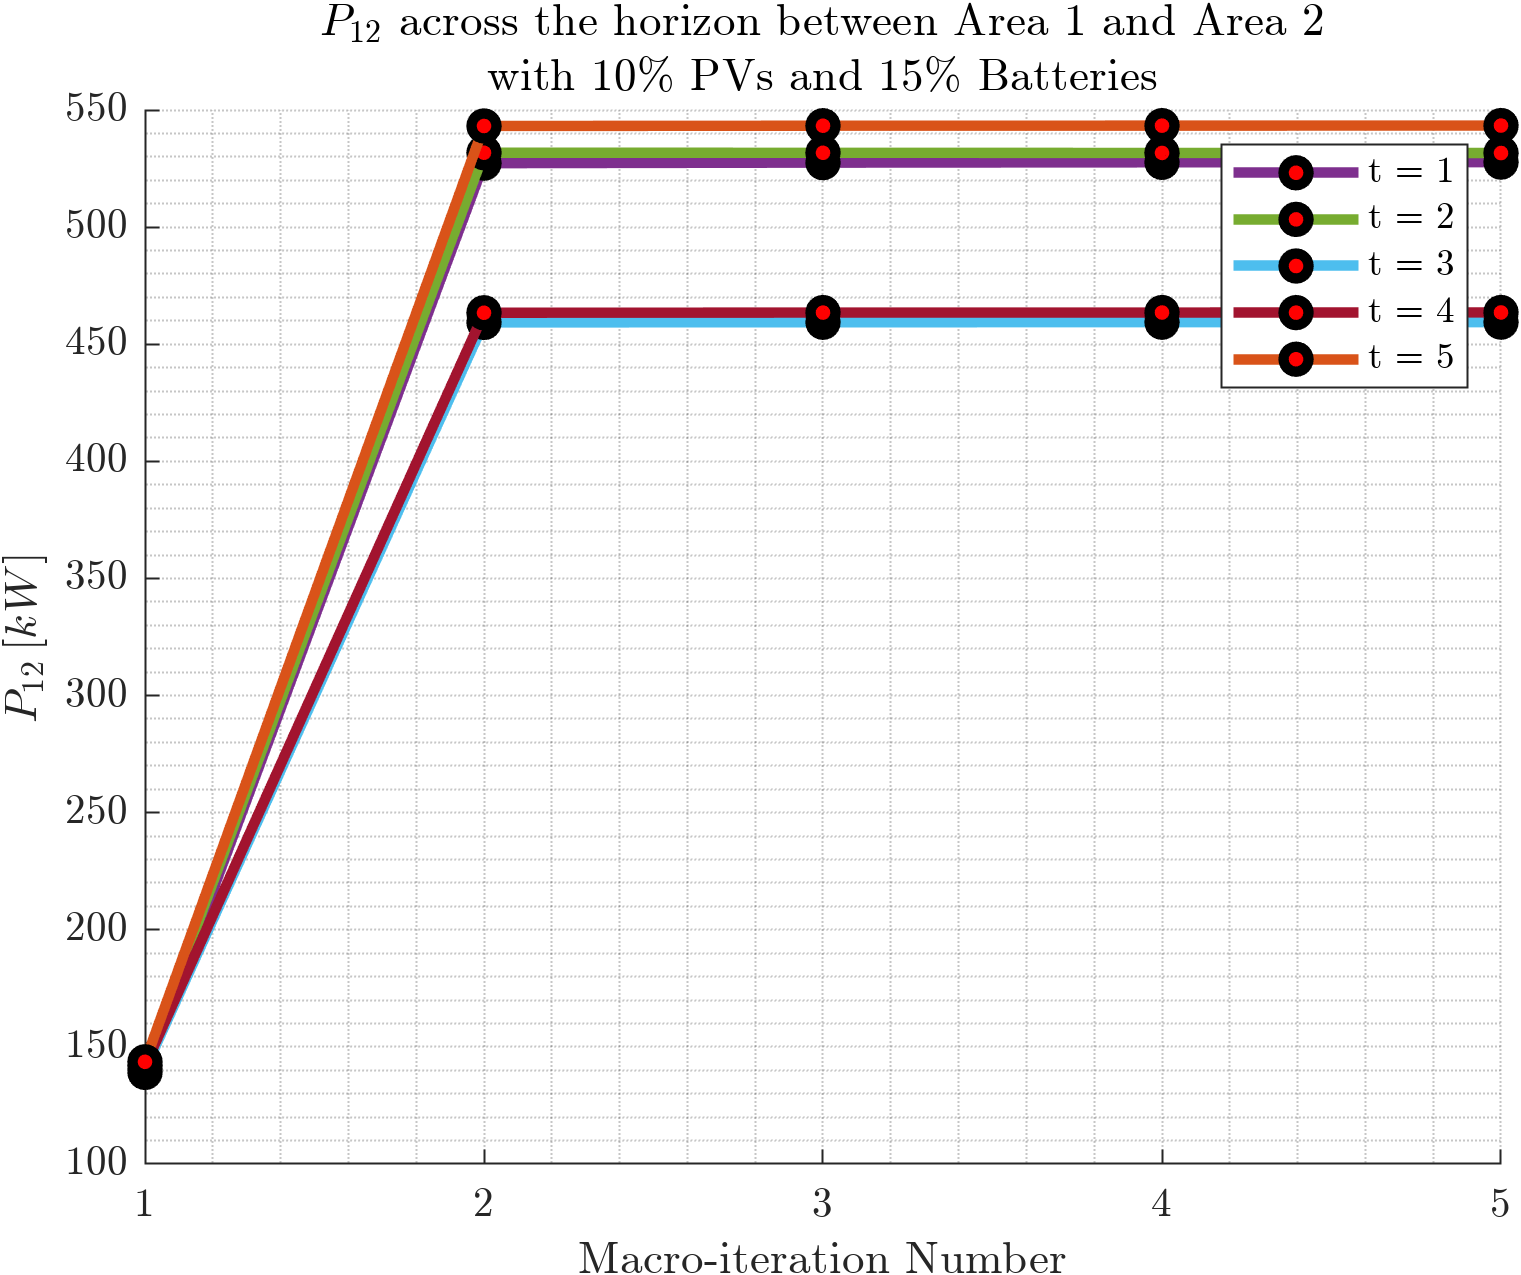
\includegraphics[width=\textwidth]{../figures/T5-pv10-batt15-PBoundary/BoundaryRealPower_vs_t_vs_macroItr_5Areas_1_2_genCost_pv_10_batt_15_.png}
        \caption{Real Power: Area 1 to Area 2}
        \label{fig:real_power_1_2}
    \end{subfigure}
    \hfill
    \begin{subfigure}[b]{0.3\textwidth}
        \centering
        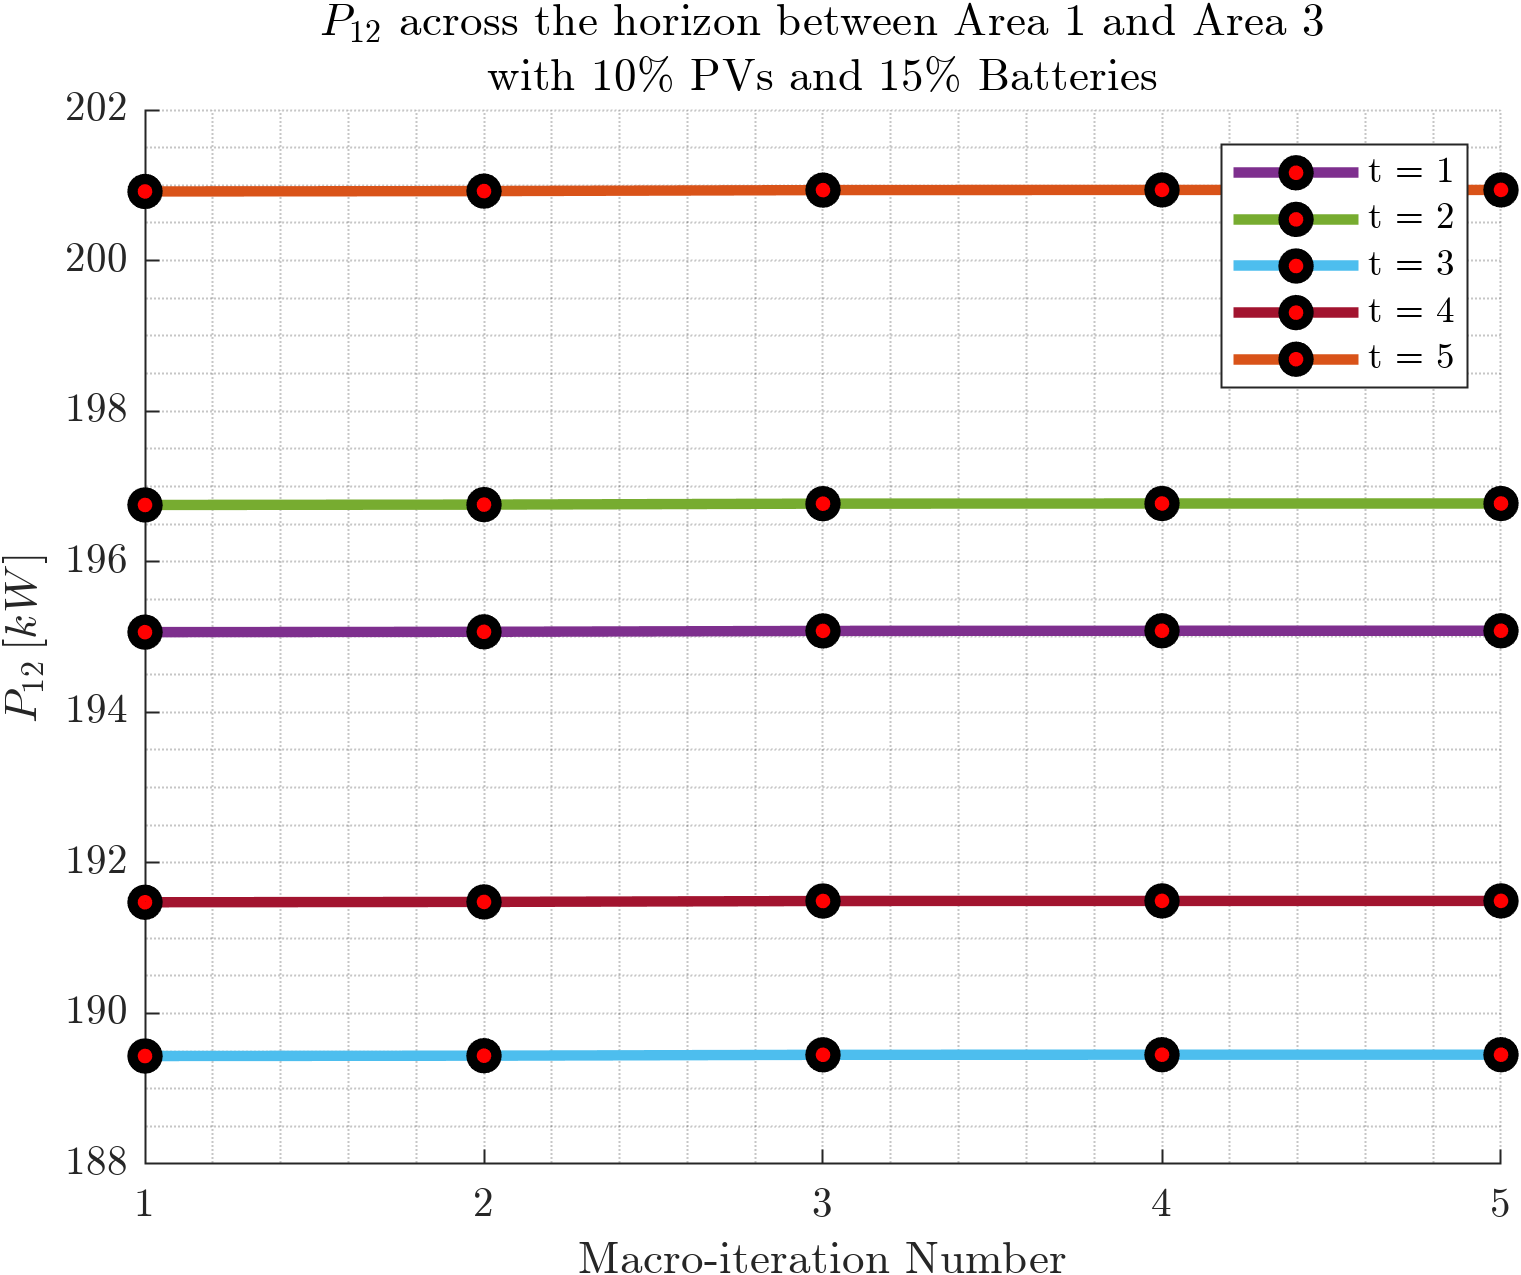
\includegraphics[width=\textwidth]{../figures/T5-pv10-batt15-PBoundary/BoundaryRealPower_vs_t_vs_macroItr_5Areas_1_3_genCost_pv_10_batt_15_.png}
        \caption{Real Power: Area 1 to Area 3}
        \label{fig:real_power_1_3}
    \end{subfigure}
    \hfill
    \begin{subfigure}[b]{0.3\textwidth}
        \centering
        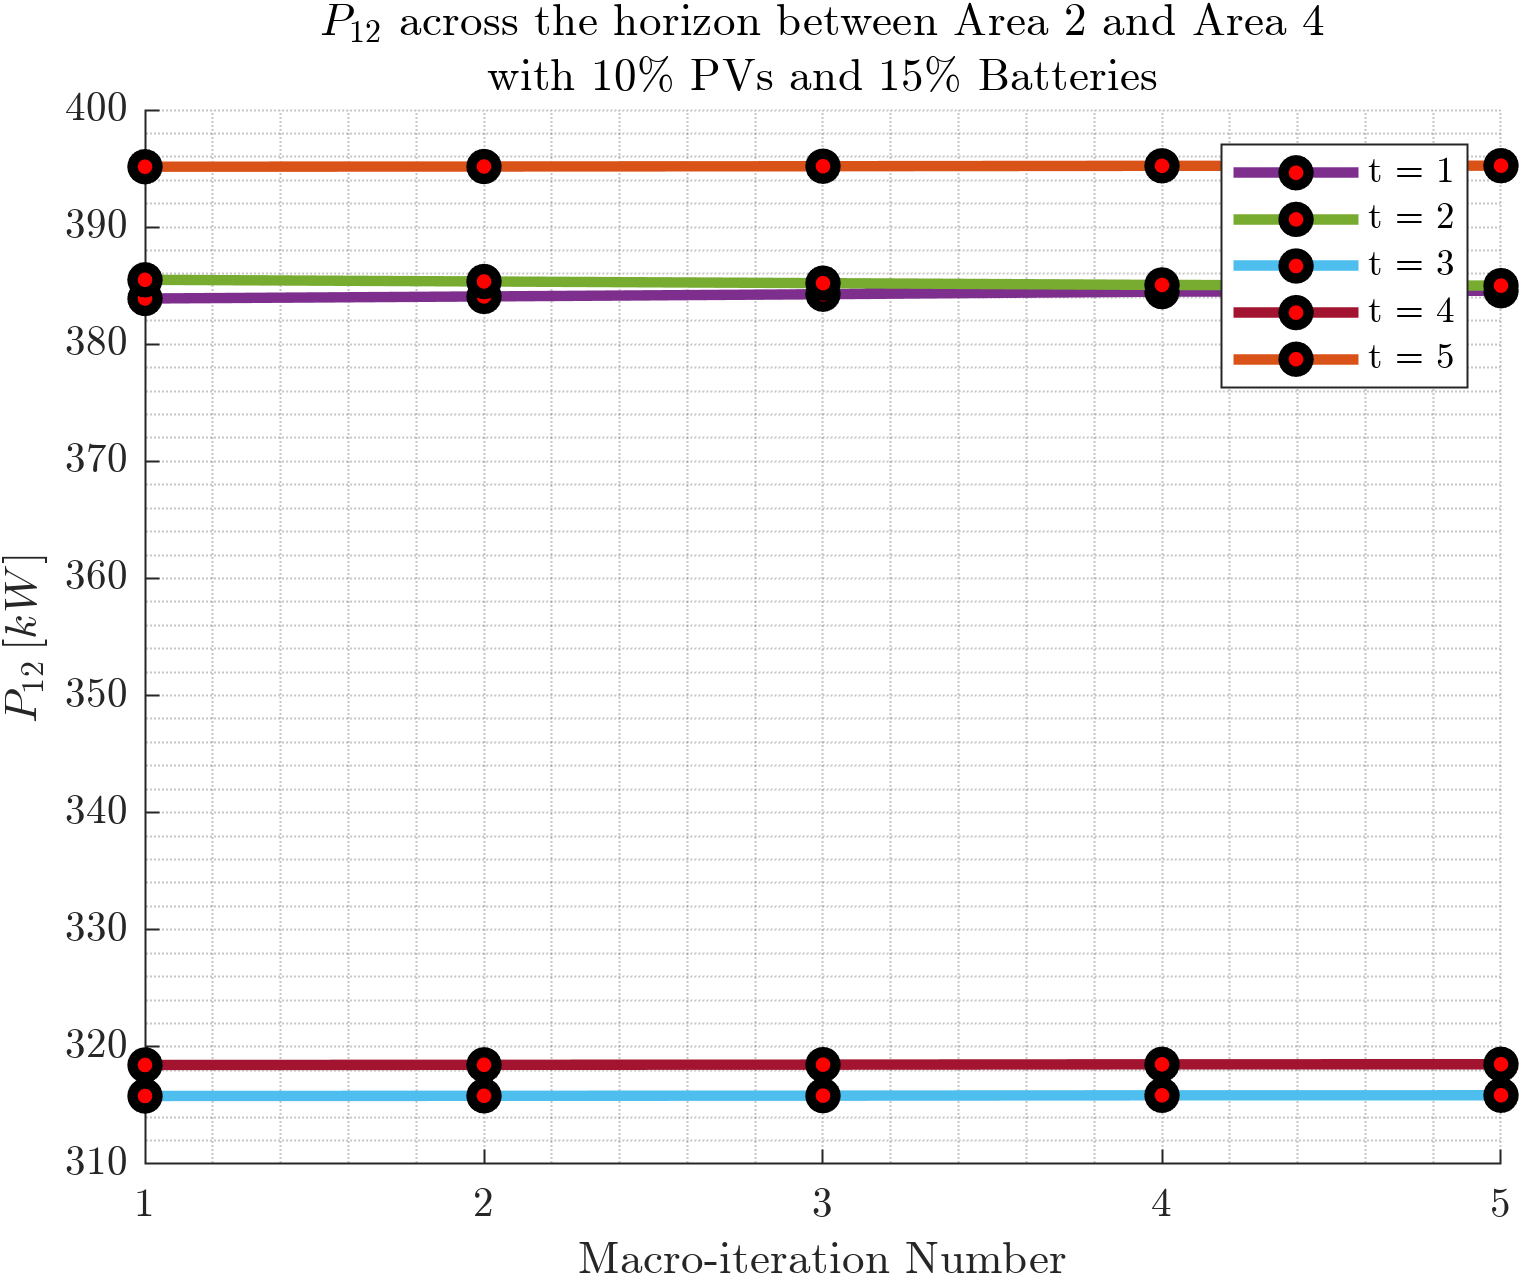
\includegraphics[width=\textwidth]{../figures/T5-pv10-batt15-PBoundary/BoundaryRealPower_vs_t_vs_macroItr_5Areas_2_4_genCost_pv_10_batt_15_.png}
        \caption{Real Power: Area 2 to Area 4}
        \label{fig:real_power_2_4}
    \end{subfigure}
    
    % Row 2
    \begin{subfigure}[b]{0.3\textwidth}
        \centering
        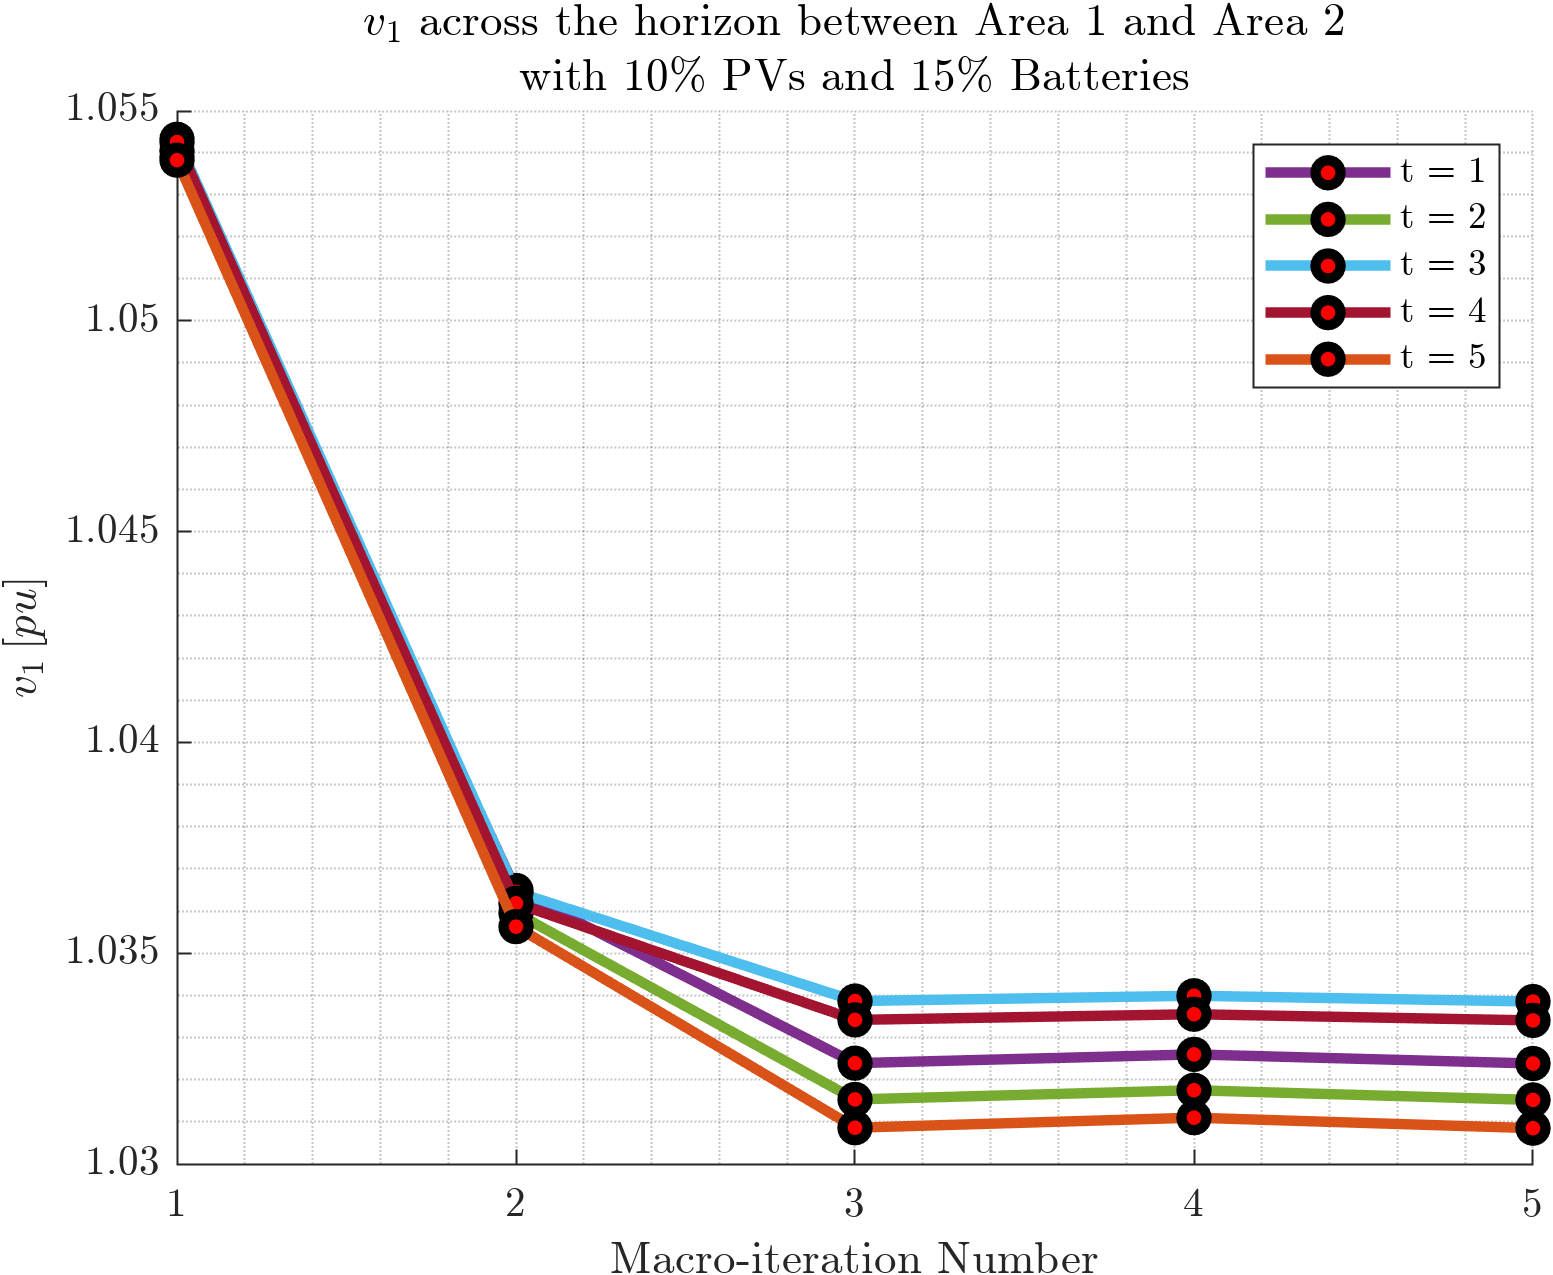
\includegraphics[width=\textwidth]{../figures/T5-pv10-batt15-vBoundary/BoundaryVoltage_vs_t_vs_macroItr_5Areas_1_2_genCost_pv_10_batt_15_.png}
        \caption{Voltage: Area 1 to Area 2}
        \label{fig:voltage_1_2}
    \end{subfigure}
    \hfill
    \begin{subfigure}[b]{0.3\textwidth}
        \centering
        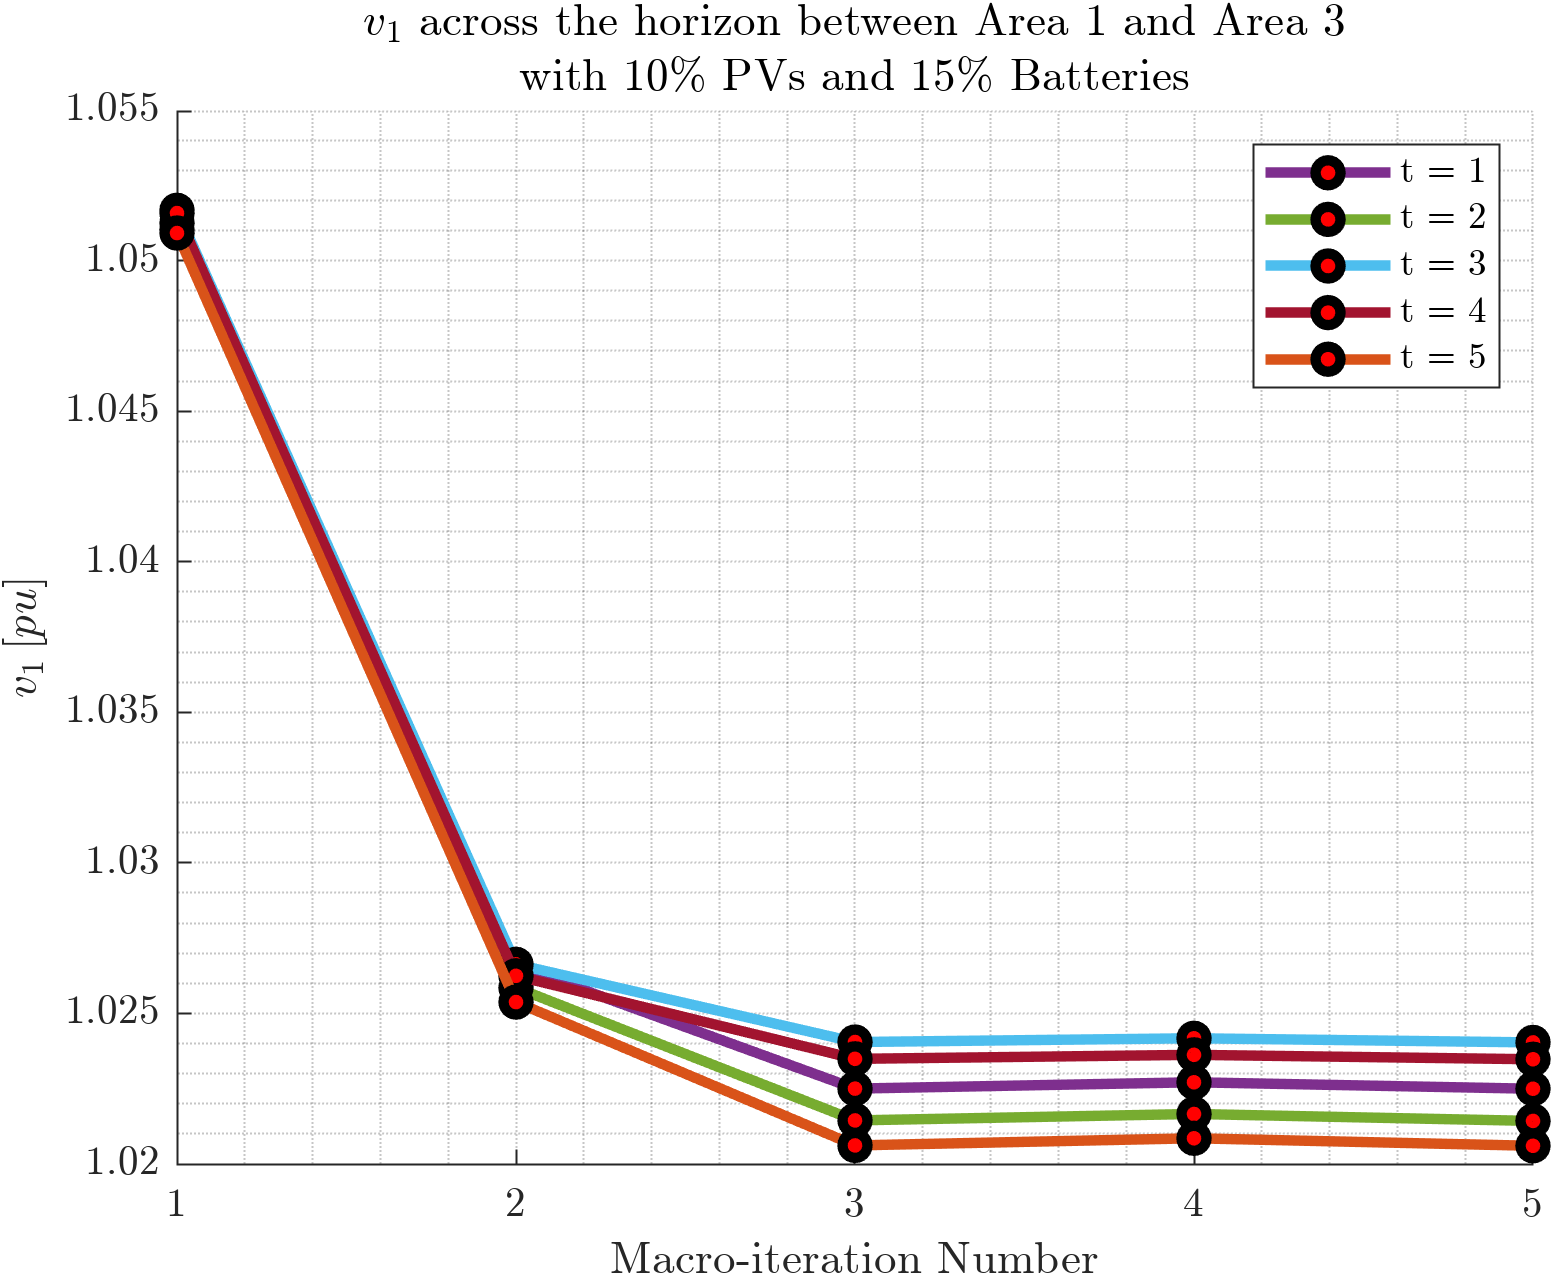
\includegraphics[width=\textwidth]{../figures/T5-pv10-batt15-vBoundary/BoundaryVoltage_vs_t_vs_macroItr_5Areas_1_3_genCost_pv_10_batt_15_.png}
        \caption{Voltage: Area 1 to Area 3}
        \label{fig:voltage_1_3}
    \end{subfigure}
    \hfill
    \begin{subfigure}[b]{0.3\textwidth}
        \centering
        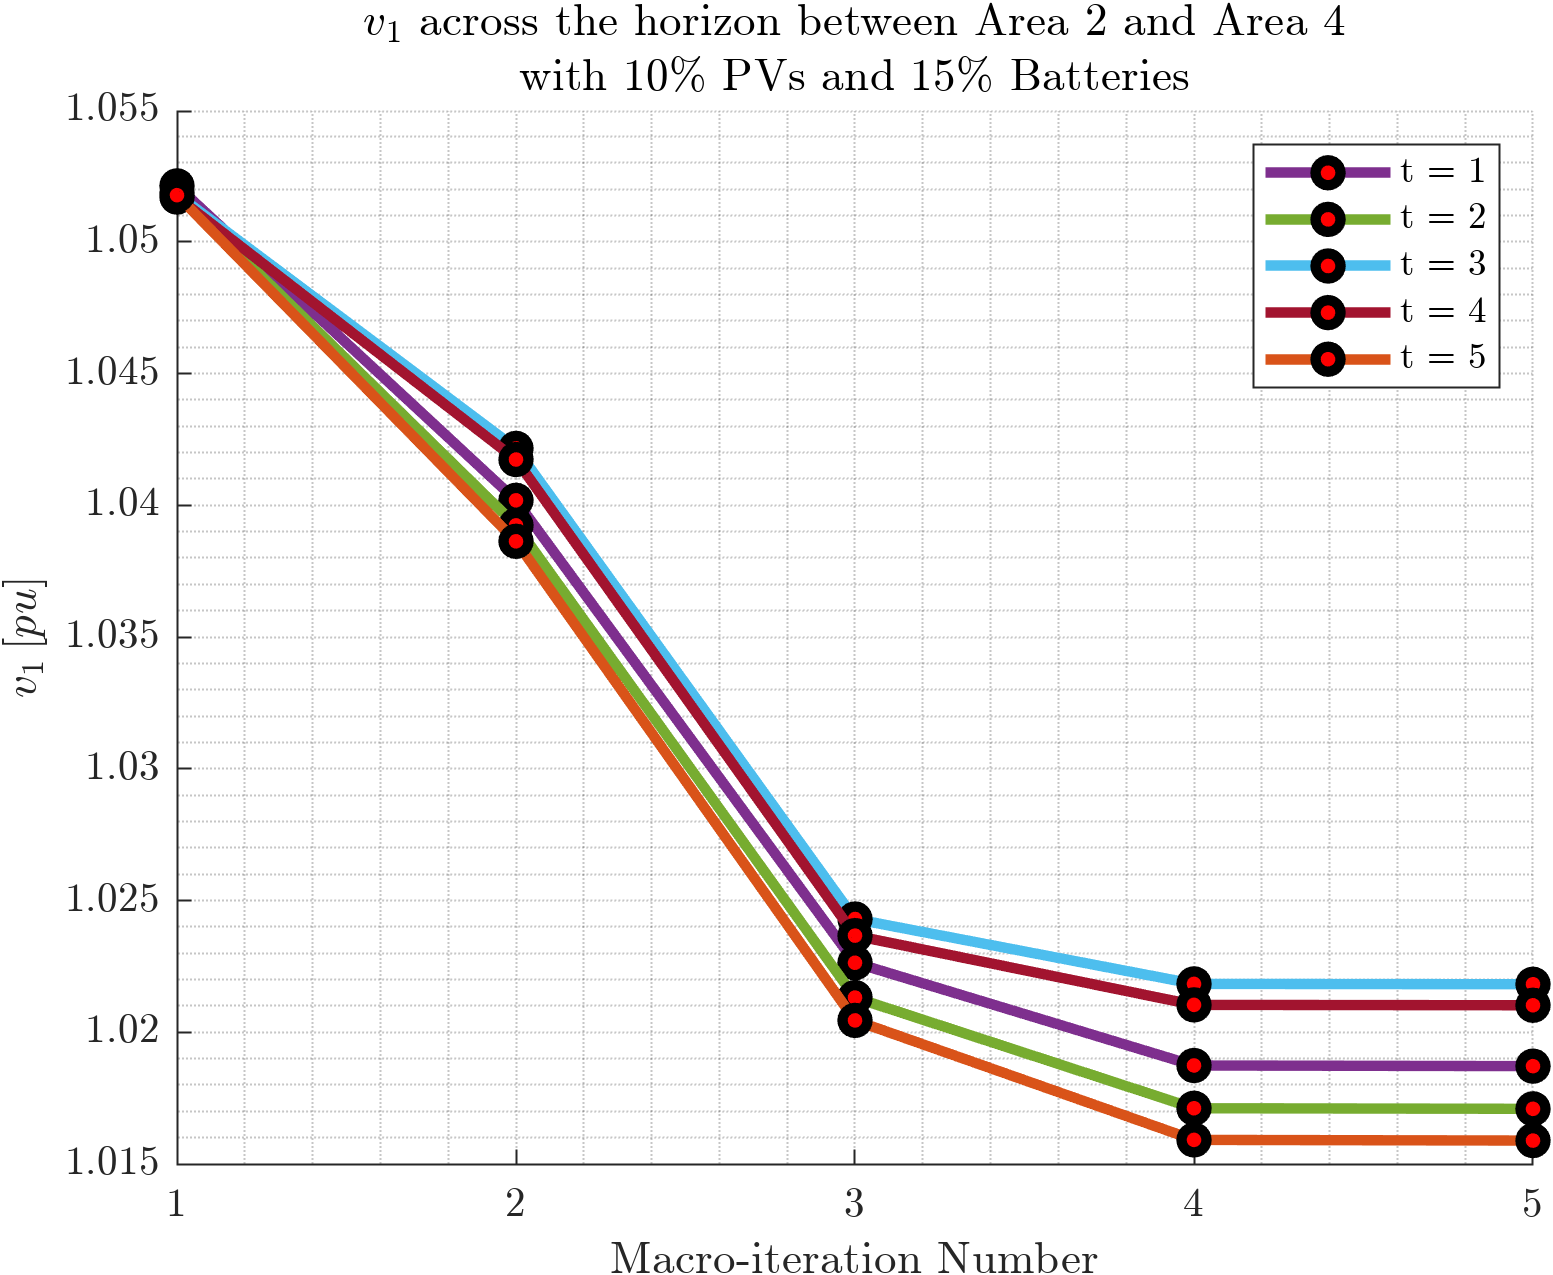
\includegraphics[width=\textwidth]{../figures/T5-pv10-batt15-vBoundary/BoundaryVoltage_vs_t_vs_macroItr_5Areas_2_4_genCost_pv_10_batt_15_.png}
        \caption{Voltage: Area 2 to Area 4}
        \label{fig:voltage_2_4}
    \end{subfigure}

    \caption{Boundary variables exchanged between pairs of areas during each iteration}
    \label{fig:boundary_variables_all}
\end{figure*}


\subsection*{IEEE 123 Node System for a 12 Hour Horizon to Demonstrate Scalability}
\begin{table}[h!]
    \centering
    \caption{Combined MPDOPF and OpenDSS Results (Substation Power Cost Minimization - 12 Hour Horizon)}
    \begin{tabular}{|l|c|c|}
    \hline
    \textbf{Metric} & \textbf{MPDOPF} & \textbf{OpenDSS} \\ \hline
    Line Loss & 194.14 kW & 194.05 kW \\ \hline
    Substation Real Power & 10595.10 kW & 10595.71 kW \\ \hline
    Substation Reactive Power & 2068.79 kVAr & 2058.30 kVAr \\ \hline
    PV Real Power & 272.60 kW & 272.60 kW \\ \hline
    PV Reactive Power & 66.04 kVAr & 66.03 kVAr \\ \hline
    Battery Real Power & -17.04 kW & -17.04 kW \\ \hline
    Battery Reactive Power & -83.30 kVAr & -83.30 kVAr \\ \hline
    Substation Power Cost & \$1424.54 & \$1424.63 \\ \hline
    Demand Real Power & \multicolumn{2}{c|}{10657.21 kW} \\ \hline
    Demand Reactive Power & \multicolumn{2}{c|}{5863.79 kVAr} \\ \hline
    \end{tabular}
    \label{table:combined_results_slim}
\end{table}

\textcolor{red}{Provide a separate graph for PV, Load forecasts for T = 5 and 12}
\begin{figure}[h!]
    \centering
    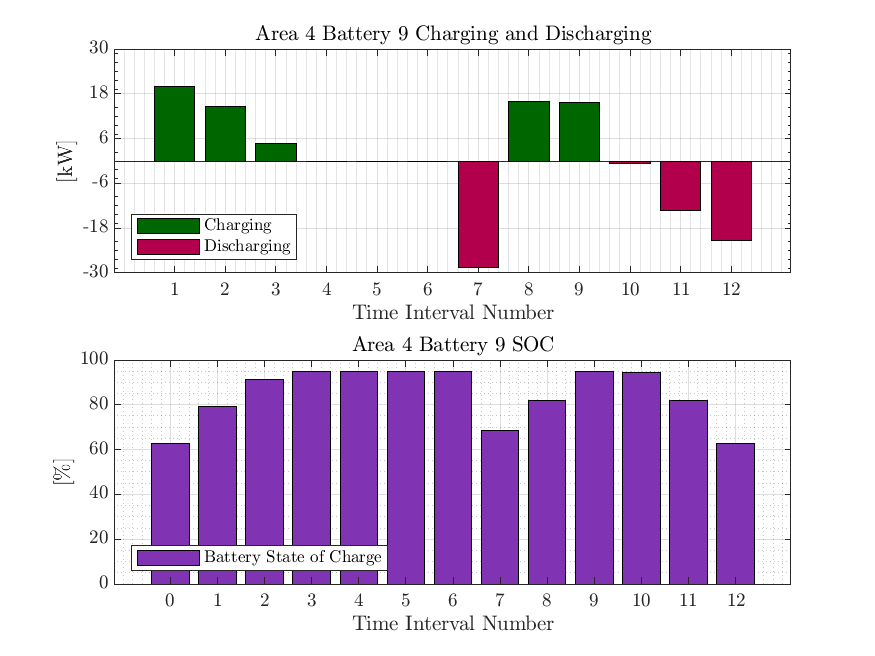
\includegraphics[width=\linewidth]{../figures/T12-pv10-batt15-genCost-peakShave/macroItr_5_genCost_peakShave_Battery_9_alpha_0.001.png}
    \caption{Charging-Discharging and SOC graphs for Battery 9 located in Area 4}
    \label{fig:battery_charging_discharging}
\end{figure}
    

\lipsum[1]

\end{document}
